{\bf Overview}\\
In brief, thus far, I have made TOAST-style pointing offset and pointing jitter operators which I have been able to run through simple (non-LAT specific) TOAST simulations. From these I can run a basic filter bin or ml mapmaker and can confirm that a simulated point source gets 'messed up'. I can also confirm that the operators adjust my pointing in the way I expect and I can run some basic beam statistics analysis on the output map (although the maps aren't themselves realistic so this was just for demonstration purposes)
I have added these operators to a local dev version of TOAST and SOTODLIB for running with the toast\_so\_sim cli so that I can model a more realistic LAT camera. This is sort of where I have hit a little wall as I have struggled to figure out how/where exactly to add the execution of my operator in the sim workflow. My toast\_so\_sim appears to run my custom operator and apply the pointing error, but the output maps are largely identical to maps with no pointing errors. I presume this is an error in how I have incorporated the custom operator into the larger simulation framework but I am still figuring that out. 

Some of my questions are specific to how to implement this in TOAST (and might not need a meeting of all of us). I also have some bigger picture questions that we should probably discuss as a group such as:

\begin{itemize}
    \item How should I be quantifying the impact of pointing errors? I was thinking I could simulate a scan of a point source and then calculate some beam statistics on the resulting map. If so, what point source? What beam stats do we care about? I presume there is existing code to do some of this for LAT beams, which code should I be using?
	\item How specifically do we want to model pointing jitter? I am currently using a sinusoidal error with gaussian noise (specifying the noise rms) as a starting point, but we should figure out if that is how we want to do things?
	\item Once I can confirm that my operator is working as intended, how should I proceed with simulating CMB observations towards the ultimate goal of using that simulated data for producing 'science'.
\end{itemize}

{\bf 2026-10-12 and 2026-10-13}\\

Today I added the basic pointing offset operator in the same way that I tried to add the pointing jitter operator as the effects of a pointing offset operator should be easier to observe than a simple pointing jitter. Claude gave me some advice as to how to properly add the new operators and make my operator more amenable to a generic TOAST sim. These changes include:
\begin{itemize}
    \item Making the operator have the option to output to a new shared key instead of overwriting the default pointing. This is so that the mapmaking scripts do not use the modified pointing, but rather the nominal pointing when trying to achieve a mapmaking solution.
    \item Making new \verb+apply_pointing_offset+ functions that can be called from the \verb+so_sim/simulate_data+ function. 
\end{itemize}

At least now I can confirm that the pointing offset operator is in fact being called, and that it is modifying the pointing as expected, as shown in the following figure.
\begin{figure}[h!]
    \centering
    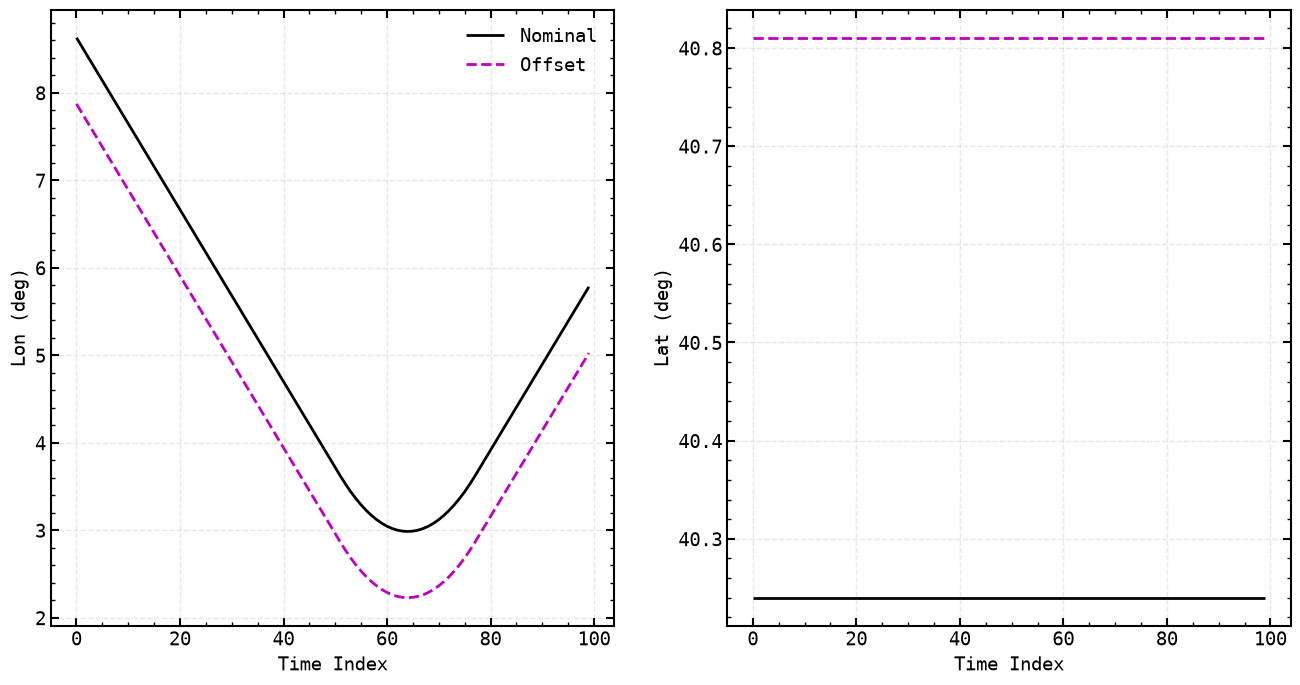
\includegraphics[width=0.8\textwidth]{Updates/figures/offset_lonlat.png}
    \caption{Pointing offset operator in action}
\end{figure}

But when I try and run the mapmaker once without offset, and once with, I still get nearly identical maps.

\begin{figure}[h!]
    \centering
    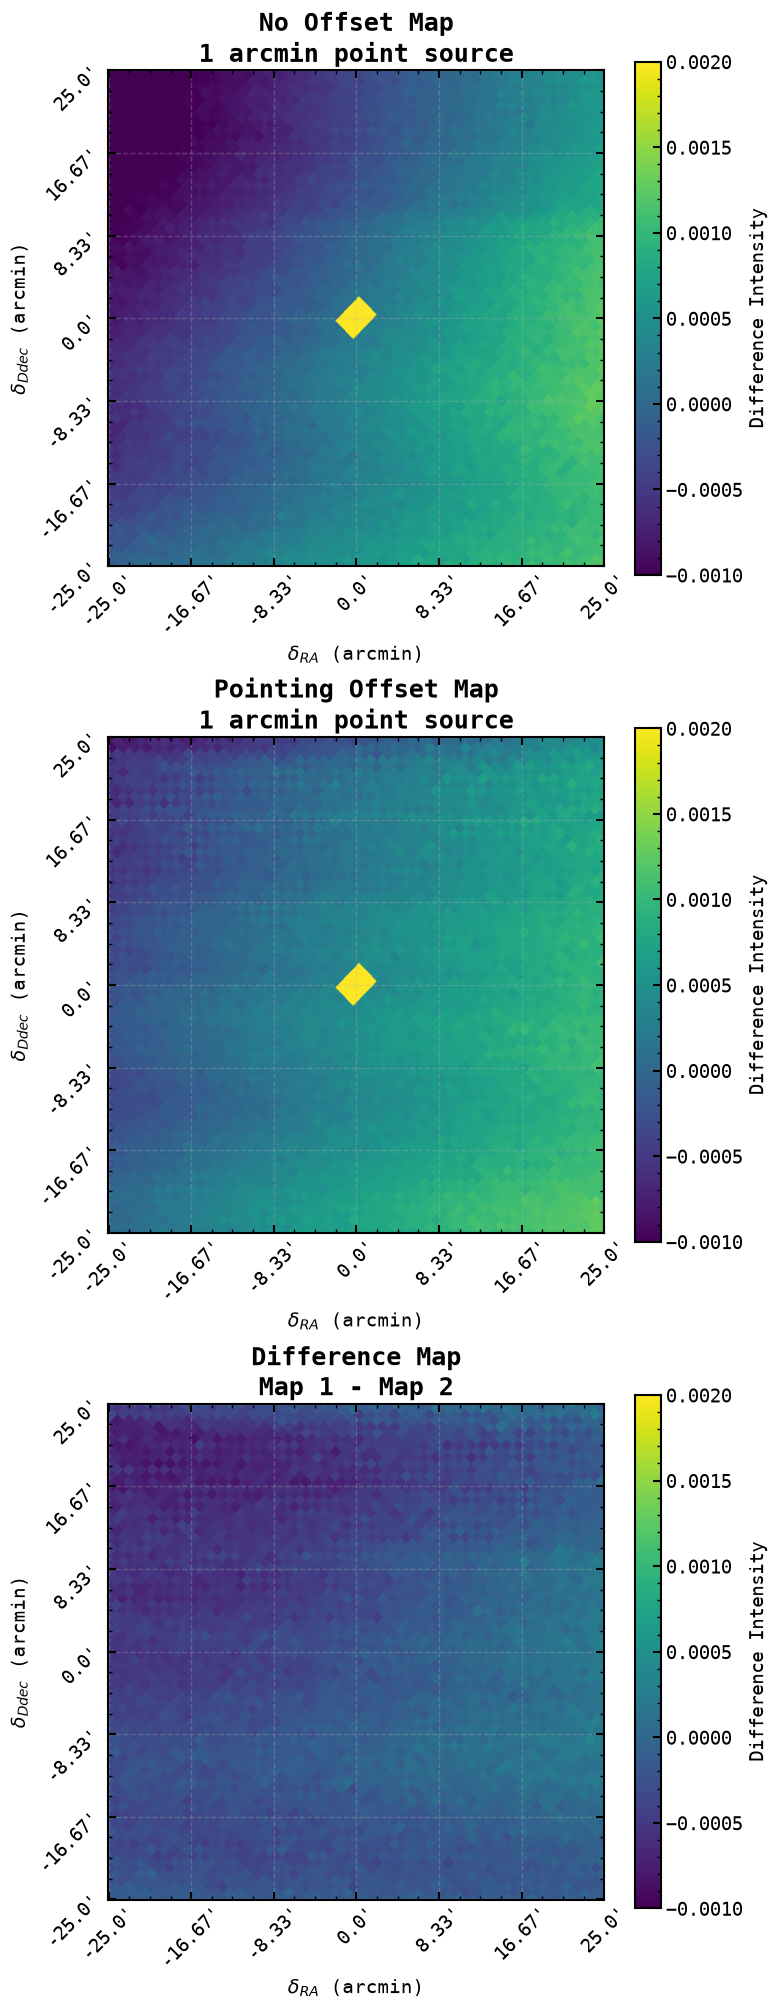
\includegraphics[width=0.5\textwidth]{Updates/figures/offset_diff_maps.png}
    \caption{Pointing offset operator in action}
\end{figure}

I am also a little concerned by the fact that my maps are not producing a sort of Airy disk pattern that I would expect from simulating a point source. I don't know if this is because of the way I am injecting a point source into my input maps, or because of how I am running the mapmaker, or something else. 